\chapter{Auditory Synthesis}
\minitoc

\begin{abstract}
We present an interactive content-based MIR environment specifically designed to aid in the exploration of databases of experimental electronic music, particularly in cases where little or no metadata exist.  In recent years, several rare archives of early experimental electronic music have become available. The Daphne Oram Collection contains one such archive, consisting of approximately 120 hours of 1/4 inch tape recordings and representing a period dating from circa 1957. This collection is recognized as an important musicological resource, representing aspects of the evolution of electronic music practices, including early tape editing methods, experimental synthesis techniques and composition. However, it is extremely challenging to derive meaningful information from this dataset, primarily for three reasons. First, the dataset is very large. Second, there is limited metadata - some titles, track lists, and occasional handwritten notes exist, but where this is true, the reliability of the annotations are unknown. Finally, and most significantly, as this is a collection of early experimental electronic music, the sonic characteristics of the material are often not consistent with traditional musical information.  In other words, there is no score, no known instrumentation, and often no recognizable acoustic source.  We present a method for the construction of a frequency component dictionary derived from the collection via Probabilistic Latent Component Analysis (PLCA), and demonstrate how an interactive 3D visualization of the relationships between the PLCA-derived dictionary and the archive is facilitating researcher's understanding of the data.
\end{abstract}

\section{Introduction}\label{sec:introduction}

We present work that attempts to facilitate researchers working on understanding the life and work of Daphne Oram through the creation of a visualization tool based on probabilistic source separation-derived models of acoustic features. 

The Daphne Oram Collection contains approximately 120 hours of 1/4 inch tape dating from approximately 1957 onwards. It is a record of the development of a number of critical techniques in music production and synthesis and includes a number of influential studio compositions, radio plays, sound effects, lectures, and interviews \cite{Young2008}.  Approximately 60 hours of the collection  has already been digitized and has been made available to researchers working on the Daphne Oram project.  However, much of the meta-data is of questionable quality, and at best difficult to verify. Furthermore, it is known that the collection contains some duplicates and several tapes feature components used by Oram in research and composition.  Among these are recordings of the Oramics machine, possibly the first synthesis and computer-composition system ever built in the United Kingdom.

There are a number of exciting content-based information retrieval challenges that this collection presents. First, what is the most effective way of making this huge collection of unknown "dark" media more available to its researchers? Secondly, how do we relate to the media given that the data itself contain almost no known instrumentation and no material that could even remotely be understood through MIDI or conventional score techniques? This is a significant issue for many collections of electronic music where timbre rather than pitch or instrument relationships are the primary composition method - there is little or no semantic information of any kind.  Thirdly, how do we locate, identify and represent extracts from the collection that might contain important recordings such as fragments of known works or recordings of the Oramics machine during its long period of development? Answering these questions is not only useful for the purposes of furthering research in musical information retrieval; it directly impacts on the research results of archivists working to understand the history and development of 20th century electronic music in Britain, of which this collection is a primary resource.

We focus on visualizing the Daphne Oram archive using two methods for describing the archive: (1) discovering latent distributions of frequencies using a recently developed source separation algorithm, probabilistic latent component analysis (PLCA) \cite{SmaragdisRajShashanka}; and (2), using a widely-adopted multi-dimensional feature for speech, music, and general acoustic classification, the Mel-Frequency Cepstral Coefficients (MFCCs).  We cluster the data from either descriptor using Multidimensional Scaling and develop a 3D visualization that allows researchers to project the archive onto multiple dimensions of the data.  Finally, we report user-feedback from researchers of the archive using the 3D visualization tool.  

Our main contribution is in describing the impact of visualizing latent timbre-relations of a large audio archive through a case-driven exploration of the work of Daphne Oram.  We compare the feedback from archivists using a visualization of latent timbre-relationships versus one using a perceptually inspired multi-dimensional feature, MFCCs, and show that PLCA is more effective at producing a meaningful visualization.  

\section{Previous Work}\label{sec:previous}

A number of previous approaches for visualizing large audio corpora have focused on the application of music-based corpora.  Some approaches to content-based musical information retrieval solutions require a user to search by example or performance, aiding retrieval when a user is unaware of exactly what they are looking for.  However, visualization of such retrieval methods often amounts to viewing lists of the $k$-most similar results of an explicit query, and thus any exploratory analysis of the corpus as a whole requires further research into approaches for visualization.  For instance, SMILE \cite{Melucci2000} presents a MIDI-keyboard for the user to ``perform'' a query, and results are presented based on how similar the MIDI sequences are to the performance.  Similar approaches built for more generic signal-based audio break a corpus into frequency information and further into fingerprints such as MFCCs or psychacoustic descriptors.  audioDB \cite{Casey2008c,Rhodes2010} for instance allows a user to input shingles, or segments of an audio track for discovering similarities in an archive.  Other solutions such as Query-by-humming allow a user to hum/sing a tune in order to discover similar results (e.g. \cite{Wang2006a,Cartwright}).  The previous methods may be suitable for applications where a user has an explicit example query.  However, in exploring an archive, it requires the user to have a priori knowledge of what the archive already contains.

Early work in exploratory content-based visualization systems can easily be traced to the 1990's where Starfields were commonly employed.  Starfields are interactive scatter-plots that allow for zooming, panning, and selection for greater detail, allowing one to view an archive through interaction.  The Informedia Digital Video Library System (1994-1998) \cite{Himmel1998,Christel1998} is one such system making use of the Starfield visualization approach, which accesses over a tera-byte of video and presents the user with an interactive scatterplot organized by the user's query.  Beginning with the audio signal, Informedia-I uses the Sphinx-II speech recognition system to discover annotations of audiovisual material.  Adding these to any existing text-annotations from captions, they create a term-document frequency matrix for each video segment, where segments are determined through the use of motion-based video-cut detection.  They are then able to discover latent relationships using PCA for reduction and visualization.  Other approaches such as IVEE \cite{Ahlberg1995} allowed for visualization options such as Tree Maps, Cone Trees, and even 3D scatterplots, though were not rooted in content-based information retrieval and instead relied on explicit relations of existing meta-data.  Though these early works were not directed for musically-based archives, their approaches towards visualization and interaction are very similar to ours, as we also look for latent relationships for reduction and visualization.

More recently, CataRT \cite{Schwarz2008} approaches Starfield style visualizations of large audio corpora by computing low-level psychoacoustic descriptors of grains segmented from a corpus for the purposes of composition, orchestration, and texture synthesis.  Visualizing the resulting mappings occurs in a 2D space where each axis is defined by a descriptor chosen by the user.  Such a visualization has the benefit of user awareness and control over the mappings that define a parametric spatial mapping.  Plumage \cite{Schwarz2008} extends the CataRT visualization into a 3D space creating a performance and composition environment where grains are colored, textured, and morphed in 3D space based on their psychoacoustic descriptions.  nepTUNE \cite{Knees2006} and \cite{Dominik2009} are two approaches to visualization which create a 3D terrain-style virtual space.  Songs are clustered using a self-organizing map of acoustic similarity in order to create virtual islands and terrain based on their clustering density.  The created virtual space thus encourages exploration and navigation of the visualized corpus.  \cite{Bartsch2001}'s approach employs the use of chroma-features for producing audio thumbnails of tracks, or segmented versions of an audio track encoding heavily repeated structures of harmonic relationships.  Though their approach is well-suited for popular music archives, they note that it is not suitable for music that does not obey a simple ``verse-refrain'' form.  \cite{Stewart2008} uses mood words to describe a 3D interactive visualization, though relies on having access to socially tagged music in order to represent the music archive.  \cite{Heise2012} use MFCCs to describe an unknown corpus of audio and explore the audio using a 2D visualization created with a self-organizing map.

The critical deviation of our approach to feature analysis from the previous approaches is by defining a 3D space using the corpora's own latent frequency distributions.  As we make no assumptions to the structure, perceptual relevance, or harmonic nature of the corpus, using probabilistic latent component analysis, we can discover the archive's own predominant distributions of frequencies and are able to use this reduced dimensionality dictionary as a representation of a high-dimensional space.  When projecting any 3-dimensions, the user is able to navigate the archive in a manner similar to CataRT \cite{Schwarz2008}. However, the axes are not user-defined psychoacoustic descriptions, but rather are projections of the archive onto ``timbres'' defined by latent frequency distributions.  Our work similarly encourages exploration and navigation as in  \cite{Knees2006,Dominik2009,Heise2012}, though takes a information-centric point of view to analysis and retrieval.   We build a second visualization using a model which does not take into account the density of the data but instead uses a perceptual frequency transformation for building decorrelated features, MFCCs, similar to \cite{Heise2012} and report the user feedback for each visualization.


%CoMIRVA, nepTUNE

% A significant research question in defining MIR browsers is how matching should be done.  A standard approach that has gained popularity from the speech community is to find the Mel-Frequency Cepstral Coefficients (MFCCs).  MFCCs are a perceptually motivated feature built using decorrelated coefficients of energy in critical bands of a frequency transform.  Soundspotter, audioDB and others are all examples of MIR-based applications that employ the MFCC.  


% AudioDB / mHashup

%SoundSpotter

%All that casey vibe.
%All the stuff on using scores/metadata and how it's useless.
%All that PLCA goodness.

\section{Method}\label{method}

Currently, the Daphne Oram Archive has over 215 tape reels or 60 hours digitized.  As the amount of available memory is a constraint on our approach, we are only able to investigate the first 10 minutes of the first 60 tape reels or 10 hours in total.  We describe each half second segment by their frequencies over time, described using the short-time Fourier transform, and describe each time-frequency matrix as a slice.  In total we have 1200 slices per tape and 72,000 slices for all 60 tape reels\footnote{We use all data for building the description of the corpus, though later use a reduced subset for visualization.}.  We aim to visualize this data using a clustering algorithm able to extract the timbre-relationships within the archive.  Specifically, we look at two methods for grouping the possible interesting frequencies describing the archive: (1) PLCA, a probabilistic method for discovering latent component relationships of a time-frequency matrix, and (2) MFCC, a widely-adopted approximation of the frequency spectrum inspired by the human auditory system's response properties.

\subsection{PLCA model}
We take an information theoretic point of view to representing an unlabeled audio archive and try to treat the problem of explaining the extracted slices from the Oram archive using a regression analysis.  Assuming there are latent distributions of frequencies that occur throughout the archive, we can aim to recover these distributions into a dictionary of frequency distributions essentially defining timbres that occur throughout the archive.  We can then discover how any slice in the archive can be explained by calculating the normalized sum of all timbres in the dictionary.  In order to do so, we make use of a recently developed model for source separation, probabilistic latent component analysis \cite{SmaragdisRajShashanka} and employ Bayesian Information Criterion-based model selection in order to automatically discover an appropriate number of components/distributions for modeling the entire archive.  

\subsubsection{Basic Formulation}
The basic PLCA model described in \cite{SmaragdisRajShashanka} treats a time-frequency matrix of magnitudes as a multinomial distribution described by a set of latent factors:
\begin{equation}\label{eq:plca}
X_{f,t} = p(f,t) \approx \sum\limits_{i}^{N}p(k_i)p(f|k_i)p(t|k_i)  
\end{equation}
where $p(f,t)$ describes the frequency $f = {1,...,R}$ versus time $t = {1,...,C}$ matrix as a probabilistic function, $k_i$ is the $i^{\mathtt{th}}$ latent component up to $N$ components, $p(k_i)$ the probability of observing the latent component $k_i$, $p(f|k_i)$, the spectral basis vector, and $p(t|k_i)$, the vector of weights over time.  Thus, the spectral basis vectors and temporal weights are described as a multinomial distribution, where the actual density of the data describes the frequency and time marginals.  The spectral basis vector is intuitively understood as the frequencies describing a particular source and the temporal weights as the envelope of sound of the source across time.  When multiplied together with their mixing weight, $p(k_i)$, they produce a 2D matrix of the source over time, while adding all $N$ matrices produces the approximation to the original matrix $X$.  

Formally discovering the marginals requires computing their maximum likelihood estimate (MLE).  This can be done iteratively through a variant of the Expectation-Maximization (EM) algorithm, a standard for estimating the MLE in latent variable models.  The E-step estimates the posterior contribution of the latent variable $k$:
\begin{equation}
p^{(t)}(k_i|f,t) = \frac{p(k_i)p(f|k_i)p(t|k_i)}{\sum_{j}^{N}p(k_j)p(f|k_j)p(t|k_j)}  
\end{equation}
The M-step then re-estimates the marginals using the posterior distribution computed in the E-step:
\begin{eqnarray}
p^{(t+1)}(k_i) &=& \sum_{f,t}\left(p^{(t)}(k_i|f,t)\frac{p(f,t)}{\sum_{f,t}p(f,t)}\right)  \\
p^{(t+1)}(f|k_i) &=& \frac{\sum_{t}p^{(t)}(k_i|f,t)p(f,t)}{p^{(t)}(k_i)}  \\
p^{(t+1)}(t|k_i) &=& \frac{\sum_{f}p^{(t)}(k_i|f,t)p(f,t)}{p^{(t)}(k_i)}  
\end{eqnarray}
One can employ a fixed number of EM iterations and assume convergence, however a least-squares or KL-divergence fit can be used to approximate the change in performance across iterations.  When the change drops below a threshold, then we assume convergence.  

\subsubsection{Model Selection}

One drawback with the basic PLCA model is the number of components describing a distribution must be known \textit{a priori}.  We therefore incorporate model selection, a commonly employed information theoretic approach to determining parameters of a model.  In the case of PLCA, the model parameters are described by $N$, the number of components.  To appropriately determine the correct value for $N$, we use \textit{Bayesian Information Criterion} (BIC) model selection.  Using the log-likelihood of the optimized parameters, an additional parameter which penalizes model complexity is subtracted from the log-likelihood:
\begin{eqnarray}
\ln{p(X)} &\simeq& \ln{p(\mathcal{D}|\theta_{\mathtt{MAP}})} - \frac{1}{2}M\ln{N}
\end{eqnarray}
where $M$ is the number of parameters in $\theta$ and $N$ is the number of data points.  BIC ensures that we do not let the model overfit to a large value of $N$, while still producing a suitable log likelihood explanation of the observed data.

To begin the model selection, we iterate through every slice of audio.  Using model selection, we compare the results of using the current number of components and using an additional component.  If the results are better explained with an additional component, we add one to the value of $N$ and continue to the next slice. Iteratively running PLCA across all slices on increasing values of $N$ until finding the maximum BIC results in finding $N=45$ for 10 hours of audio.  

\subsection{MFCC Model}
For our second model, we use the commonly employed Mel-frequency Cepstral Coefficients (MFCCs) which approximates a frequency spectrum by a set of de-correlated features.  For completeness sake, we summarize the basic algorithm of computing MFCCs below:

\begin{enumerate}[noitemsep]
\item Window the input audio signal and take the discrete Fourier transform
\item Warp the absolute power spectrum into $M$ triangular sub-bands, spaced equally on the Mel-frequency scale with 50\% overlap.  The following approximate formula describes a frequency on the Mel-frequency scale given an input linear frequency:
\begin{equation}
mel(f) = 2595*\log_{10}{1+\frac{f}{700}}
\end{equation}
Using this mapping, warp the power spectrum to the Mel-scale and compute the energy in each sub-band as follows:
\begin{equation}
S_m = \log{\left(\sum_{k=0}^{N-1}|X[k]|^2H_m[k]\right)}
\end{equation}
where $H_m$ are the filter-banks described by the Mel-frequency scale.
\item Finally, we compute the discrete cosine transform to obtain the first $C$ MFCCs:
\begin{equation}
c_n = \sqrt{\frac{2}{M}}\sum_{m=1}^{M}(S_m\times\cos{[n(m-\frac{1}{2})]}\frac{\pi}{M}
\end{equation}
and $n = 1,...,C$, where $C$ is the number of coefficients to return (discarding high-frequency coefficients), and $M$ is the number of triangular sub-bands.
\end{enumerate}

For our purposes, we use a standard decomposition of $M=40$ triangular bands and keep $C=13$ coefficients.

\subsection{Multi-dimensional Scaling}
After running each model, we are left with an $M \times N$ dimensional matrix, where $M$ refers to the number of time slices, and $N$ to the number of dimensions that describe each feature.  In the case of PLCA, after running model selection, we are left with $N=45$ dimensions describing the data.  With regards to MFCCs, we specifically choose $N=13$ cepstral coefficients.  

In order to visualize the high-dimensional space created by either model and cluster together similarly weighted features, we make use of Multi-Dimensional Scaling (MDS), a popular technique for multivariate and exploratory data analysis. MDS is a common technique for projecting data in high-dimensional spaces to 2 or 3 dimensional spaces for the purposes of visualization.  It aims to preserve the pairwise distances between data points, starting with the notion of distance, and working backwards in order to create the coordinate space.  The basic algorithm for calculating the unknown low-dimensional coordinate map $\mathbf{X}$ thus starts with a distance or proximity matrix, $\mathbf{P}$.  We aimed to use the full archive of 72,000 slices, however creating a matrix of float values this large requires $~20$ gigabytes of information which must be held in RAM.  Therefore, we reduce our database by taking every 5th slice, effectively looking at 0.5 second slices every 2.5 seconds rather than every 0.5 seconds.  However, the description of the data in the case of PLCA is still dependent on all 72,000 slices.
  
In order to calculate the low-dimensional coordinate matrix, we calculate the largest eigenvalues of the distance matrix after applying a double centering procedure.  The basic MDS algorithm is summarized as follows:
\begin{enumerate}[noitemsep]
\item Compute a $M \times M$ proximity matrix $\mathbf{P}$ by calculating the Euclidean distances between each of the $M$ features
\item Compute the inner product matrix $\mathbf{B}$ by applying double-centring to the proximity matrix $\mathbf{P}$: 
\begin{equation}
\mathbf{B} = -\frac{1}{2}\mathbf{J}\mathbf{P}^{(2)}\mathbf{J}
\end{equation}
where $\mathbf{J} = \mathbf{I} - n^{-1}\mathbf{1}\mathbf{1^{\mathtt{T}}}$ and $n$ is the number of objects.
\item Compute the eigenvalue decomposition and retain the $n$ largest eigenvectors, $\mathbf{e}_1, ..., \mathbf{e}_n$ in order to compute the $n$-dimensional coordinate matrix $\mathbf{X}$:
\begin{equation}
\mathbf{X} = \mathbf{E}_n\mathbf{\Lambda}_n^{\frac{1}{2}}
\end{equation}
using the eigenvectors $\mathbf{E}$ and eigenvalues $\mathbf{\Lambda}$ of $\mathbf{B}$ 
\end{enumerate}

One may also notice the algorithm is equivalent to a doubly-centered version of PCA in the case where the distances are Euclidean.  As both the PLCA and MFCC model's feature dimensions are de-correlated, we would expect to find the number of eigenvalues approach the same dimensionality as either model.  Thus, the PLCA model is clustered in 45 dimensions, and the MFCC model in 13.


\section{Browser}

\begin{figure*}
  \centering
  \label{fig:gui}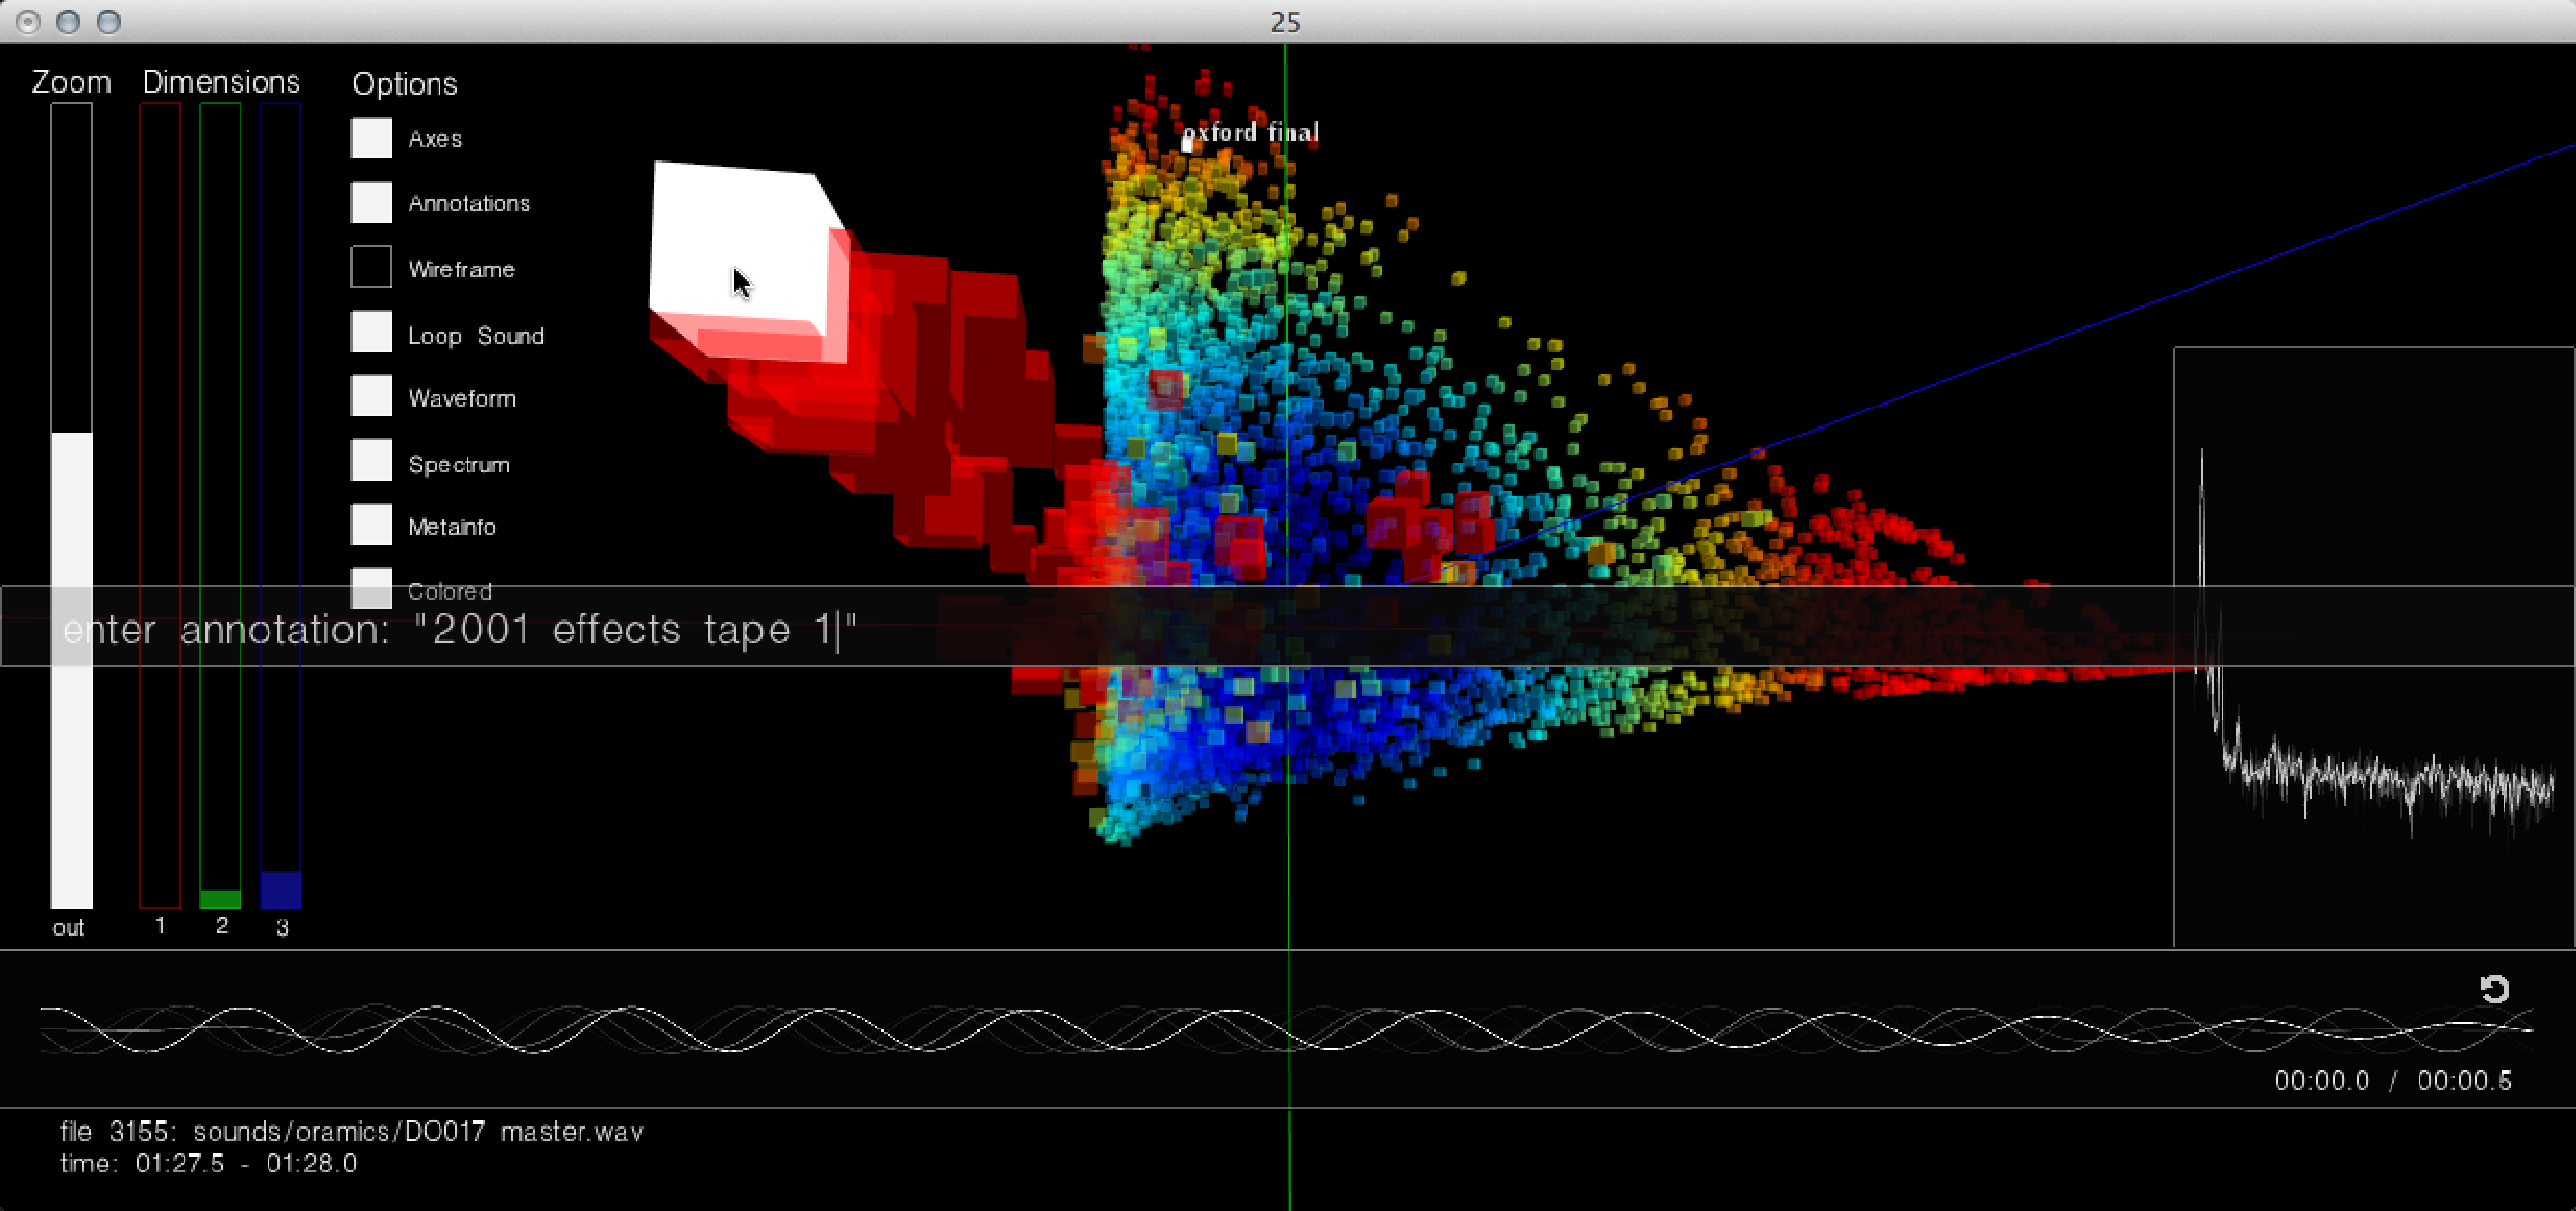
\includegraphics[width=0.99\textwidth]{images/gui.pdf}
  \caption{Screenshot depicting the GUI of the browser (best viewed in color).  Here a user is currently inputing text in order to annotate one of the sound segments.  We can see sliders to the left allowing the user to zoom in/out, change the dimensions of the visualization, and control which elements are drawn on screen.  With all of the options being drawn, we see the waveform of the currently highlighted sound (depicted with a white cube under the mouse cursor) is drawn on the bottom.  As well, the meta-data describing the file name is just below the waveform.  To the right, the decibel-scale spectrum is also drawn.  All elements are drawn in real-time and are interactively manipulated in 3D space.}
\end{figure*}

The interface is shown in Figure \ref{fig:gui} and is built in C/C++ using the creative-coding toolkit openFrameworks\footnote{http://www.openframeworks.cc}.  The user is presented with a 3D space (see Figure \ref{fig:gui}) where each slice of sound from the archive is represented as a cube projected in 3D space.  The coordinates of the cube are determined by which dimensions of the MDS coordinate matrix are selected.  To begin, the first three dimensions are displayed.  Users can then select any dimension to be displayed on the 3-axes.  As a result, the visualization can also be constrained to a 2D visualization by simply choosing the same dimension for 2 axes.  A colormap is used to help depict distance from the OpenGL origin (using a ``jet'' colormap, i.e.: blue-yellow-red), though the user can turn this off.  Figures \ref{fig:plca} and \ref{fig:mfcc} depict the visualizations  of the first three dimensions produced using MDS inside the browser.  

While inside the browser, pressing space-bar allows one to annotate the currently selected slice.  The annotated text appears in 3D next to the slice's cube.  The slice's audio is also visualized as a waveform and its instantaneous Fourier transform.  As we used the first ten minutes of every tape-reel, the waveform for any given slice is presented as a looped region within a 10 minute audio file.  However, the user can change the loop regions to hear any other portion of the original audio file while selecting a slice, thus allowing the user to listen to the audio before and after the slice.

The user can also move the camera around the OpenGL origin by dragging the left mouse button in the 3D space.   Highlighting any of the cubes with the mouse allows the user to inspect the clip in greater detail.  Taking a cue from the 2D analog CataRT, any of the cubes can be ``scrubbed'' for playback by simply moving the mouse over any of the cubes, not requiring any further interaction to listen to the sound sample.  Zooming in and out of the 3D space can be done via the mouse scroll wheel or graphical slider.  Double-clicking on any of the cubes re-centers the origin to the selected cube, allowing camera interaction to occur with respect to the cube.  Cubes can be spaced closer or farther from each other using another graphical slider.  This allows more tightly clustered portions of a visualization to be explored in greater detail.  

%Describe how you derived the PLCA model
%Describe how you derive the MFCC model
%Descirbe the MDS stuff
%Describe how you created the visualisation
%Describe the user studies and how the interface evolved
%State that we worked with the users to make the interface more usable.


\section{User Feedback}\label{results}

Three researchers of the Oram Archive were invited to navigate the browser and spent 1 hour in total using both the PLCA and MFCC visualizations.  They were unaware of how either model was created, were unfamiliar with signal processing and machine learning, and were only told that we are investigating a way to navigate the Oram Archive.  Each user was given 5-10 minutes of explanation of the features of the browser and were then left to explore the browser by themselves.  Each user proceeded to explore the archive by using the mouse to listen to the different slices located in 3D space.  In addition, each user managed to find particularities of the archive that seemingly would have been very difficult without the browser.  For instance, finding a significant portion of one tape reel that was labeled as ``POP TRY-OUTS'' in another reel labeled as ``COPY DONKEY HELL ABC \& ITV. BIRDS \& PERC'' by exploring slices located near each other in the 3D space.  Also, one found components relating to Daphne Oram's piece, ``Birds of Parallax'' during lectures series that were only labeled by their location, indicating she demonstrated these components during her talk.

When asked to compare the two visualizations and remark on their usability as a navigation tool of the Daphne Oram Archive, the three researchers reported on the form of the MFCC model in comparison to the PLCA one, saying (1), ``it has a less useful shape in general'', (2) ``it has less detail'', and (3) ``this dense mass represents total variety...and I don't quite understand how it is mapped.''  In response, we asked what if anything made the PLCA model more useful for navigation in comparison to the MFCC model.  User 1 reported: ``it has a more definite and understandable space. For example, prongs that have specific information in them such as silence.'' and User 3 reported: ``Oh that's really successful, it seems to be matching pitch and you start to see how she was using pitch'' and ``I had a clear sense of how it was mapped''. 

Each user also gave many helpful possible extensions to the current functionality of the browser, including the ability to save camera states, only view a particular reel's slices, and auto-zoom and rotation around a particular point.  User 1 found the 3D nature of the visualization required more practice saying they ``might get used to it'' while User 3 commented on navigating around a single slice saying ``I understand it as a structure, but I'm working out where in 3D space [the slice] is.  You have to move around in 3D before working it out.''   User 3 also expressed the scope of the browser for new users to see and appreciate Daphne Oram's work, remarking, ``Goes to show just how much variety there are in the samples, and this has made that variety accessible.''  

User 2 additionally remarked on the potential of incorporating other mediums of Daphne's work saying it would be great to ``include other mediums than audio, combining with video/letters/images.''  As well, both User 2 and User 3 commented on the tool's applicability to performance and composition, saying he/she was ``fascinated as a compositional tool.  Navigating different dimensions, it's a beautiful instrument'' and ``it is nice to categorize sounds as it is what we do in sampling''.  

\begin{figure}
  \centering
  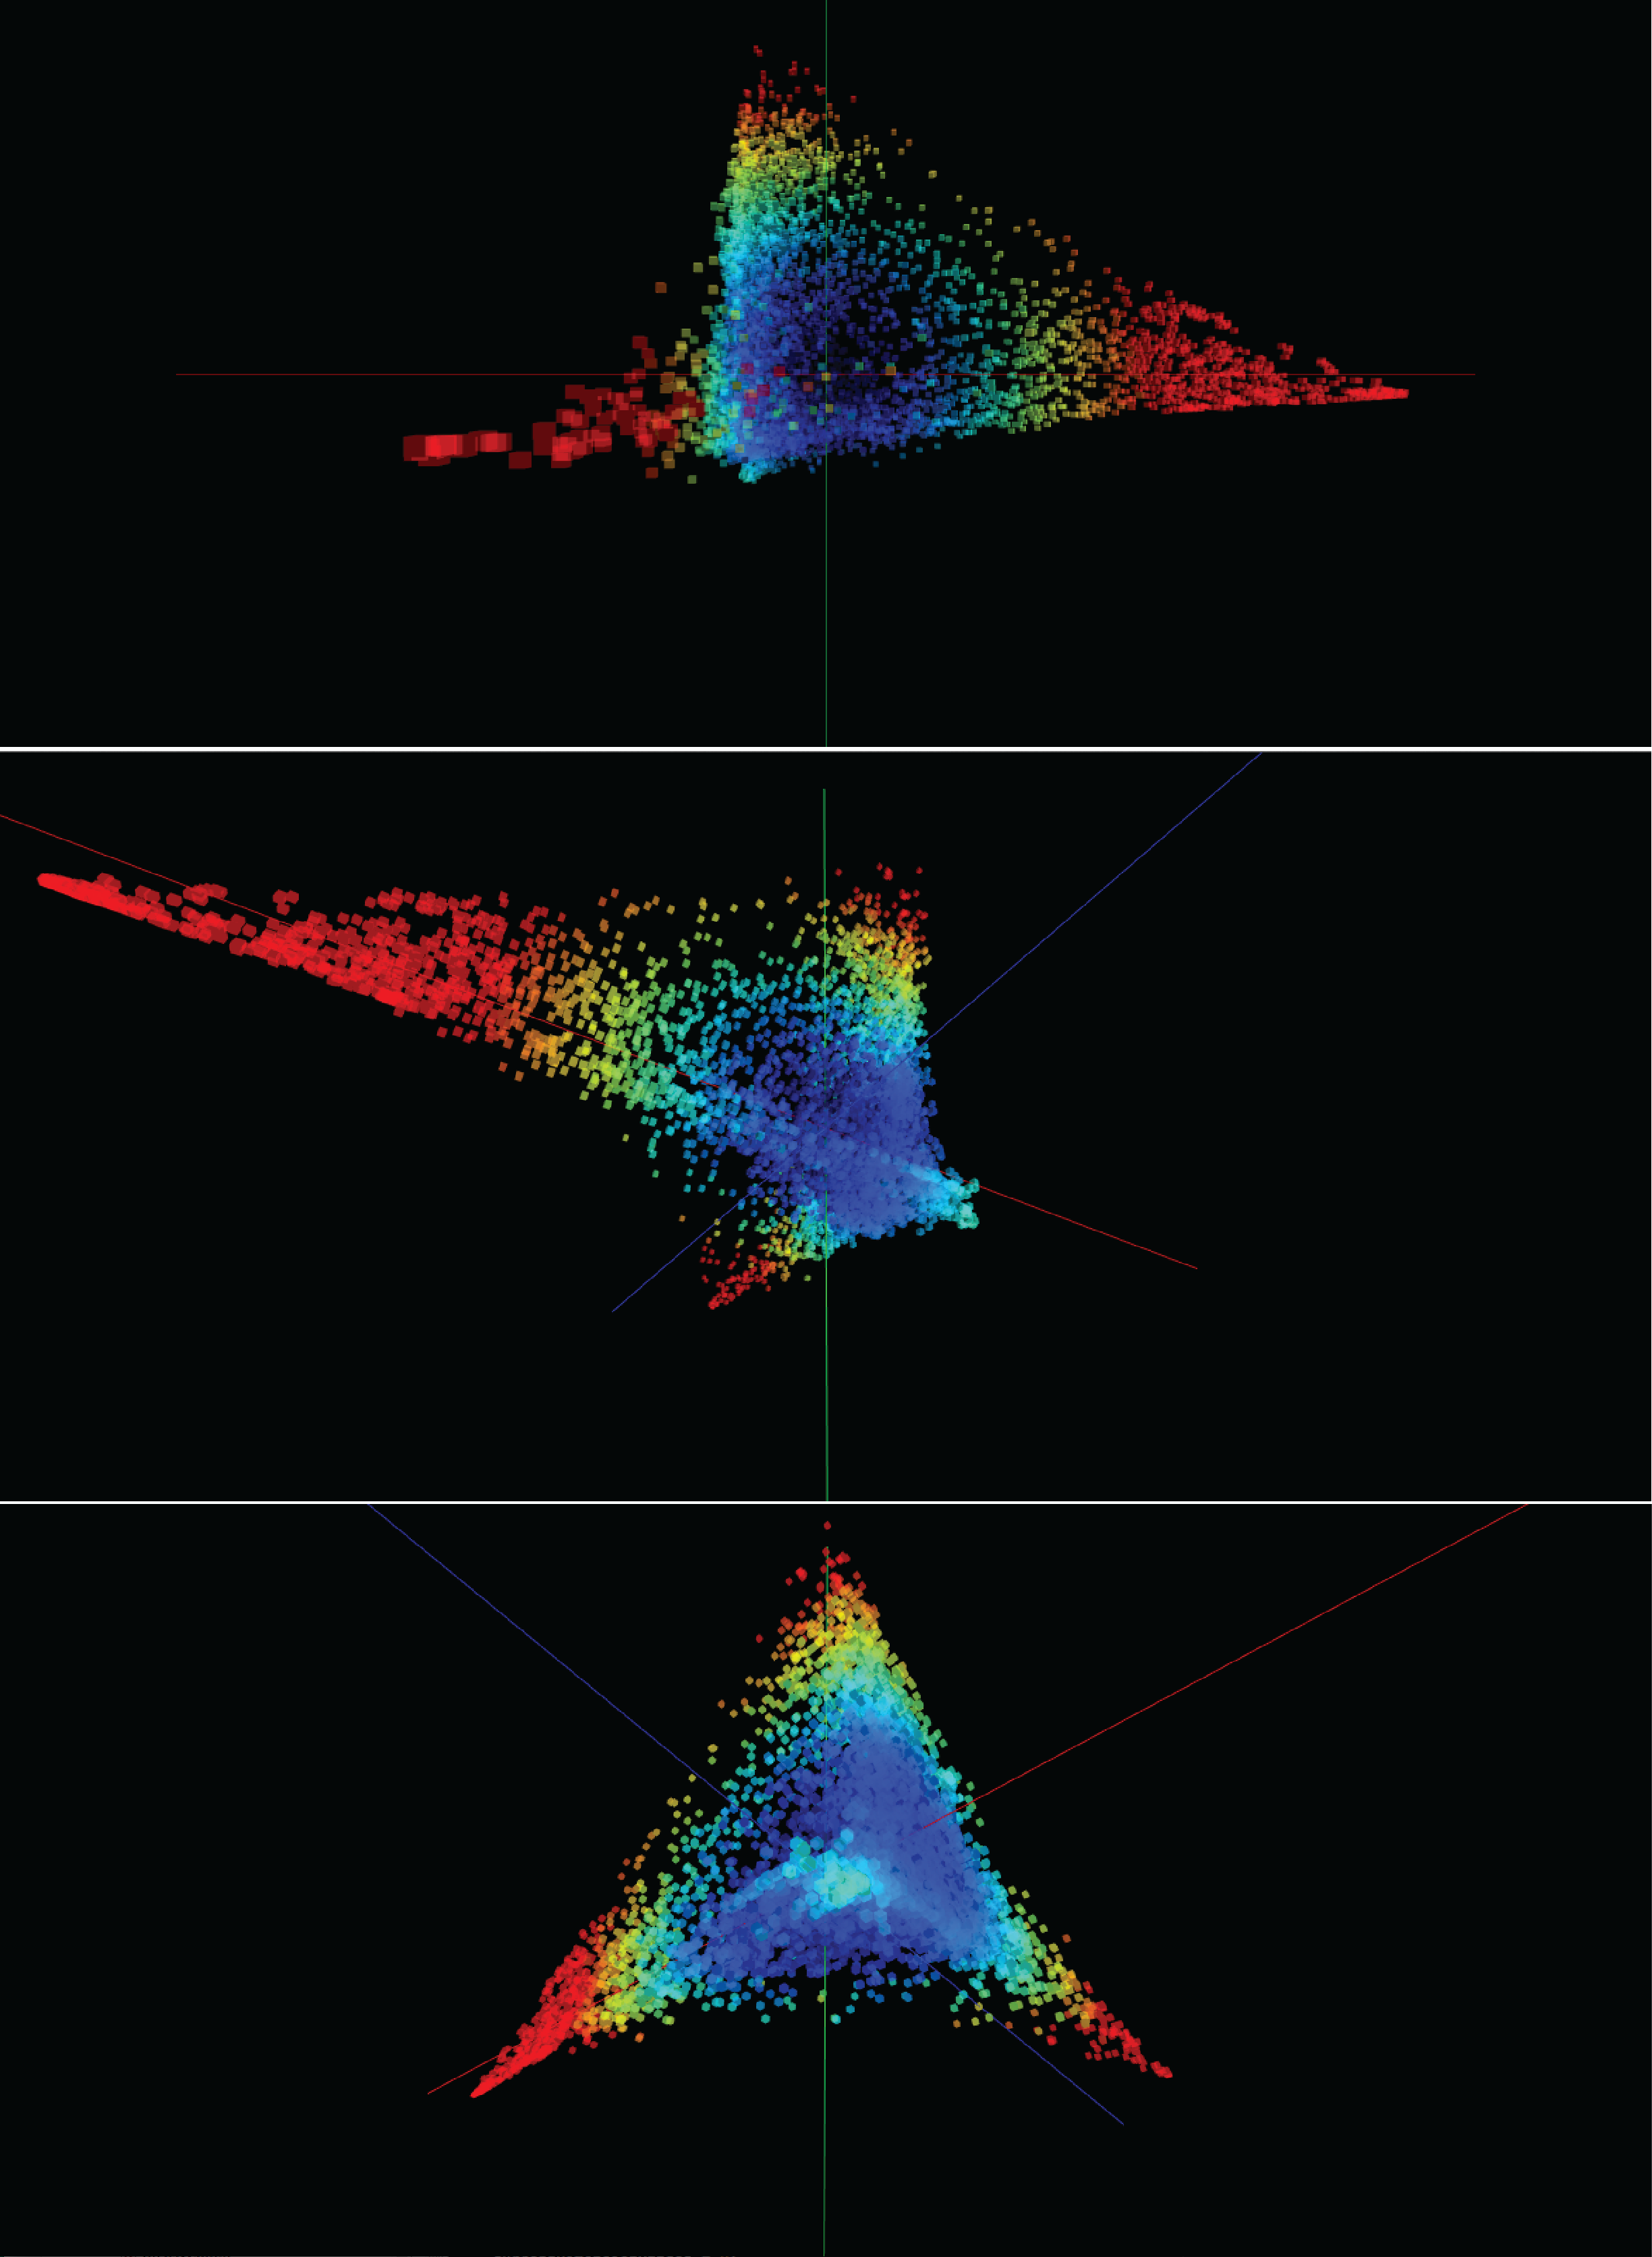
\includegraphics[width=0.38\textwidth]{images/plca-all.png}
  \caption{Screenshot of the first 3 dimensions of the PLCA model visualized in the browser.  We show three different views here.}
  \label{fig:plca}
\end{figure}

\begin{figure}
  \centering
 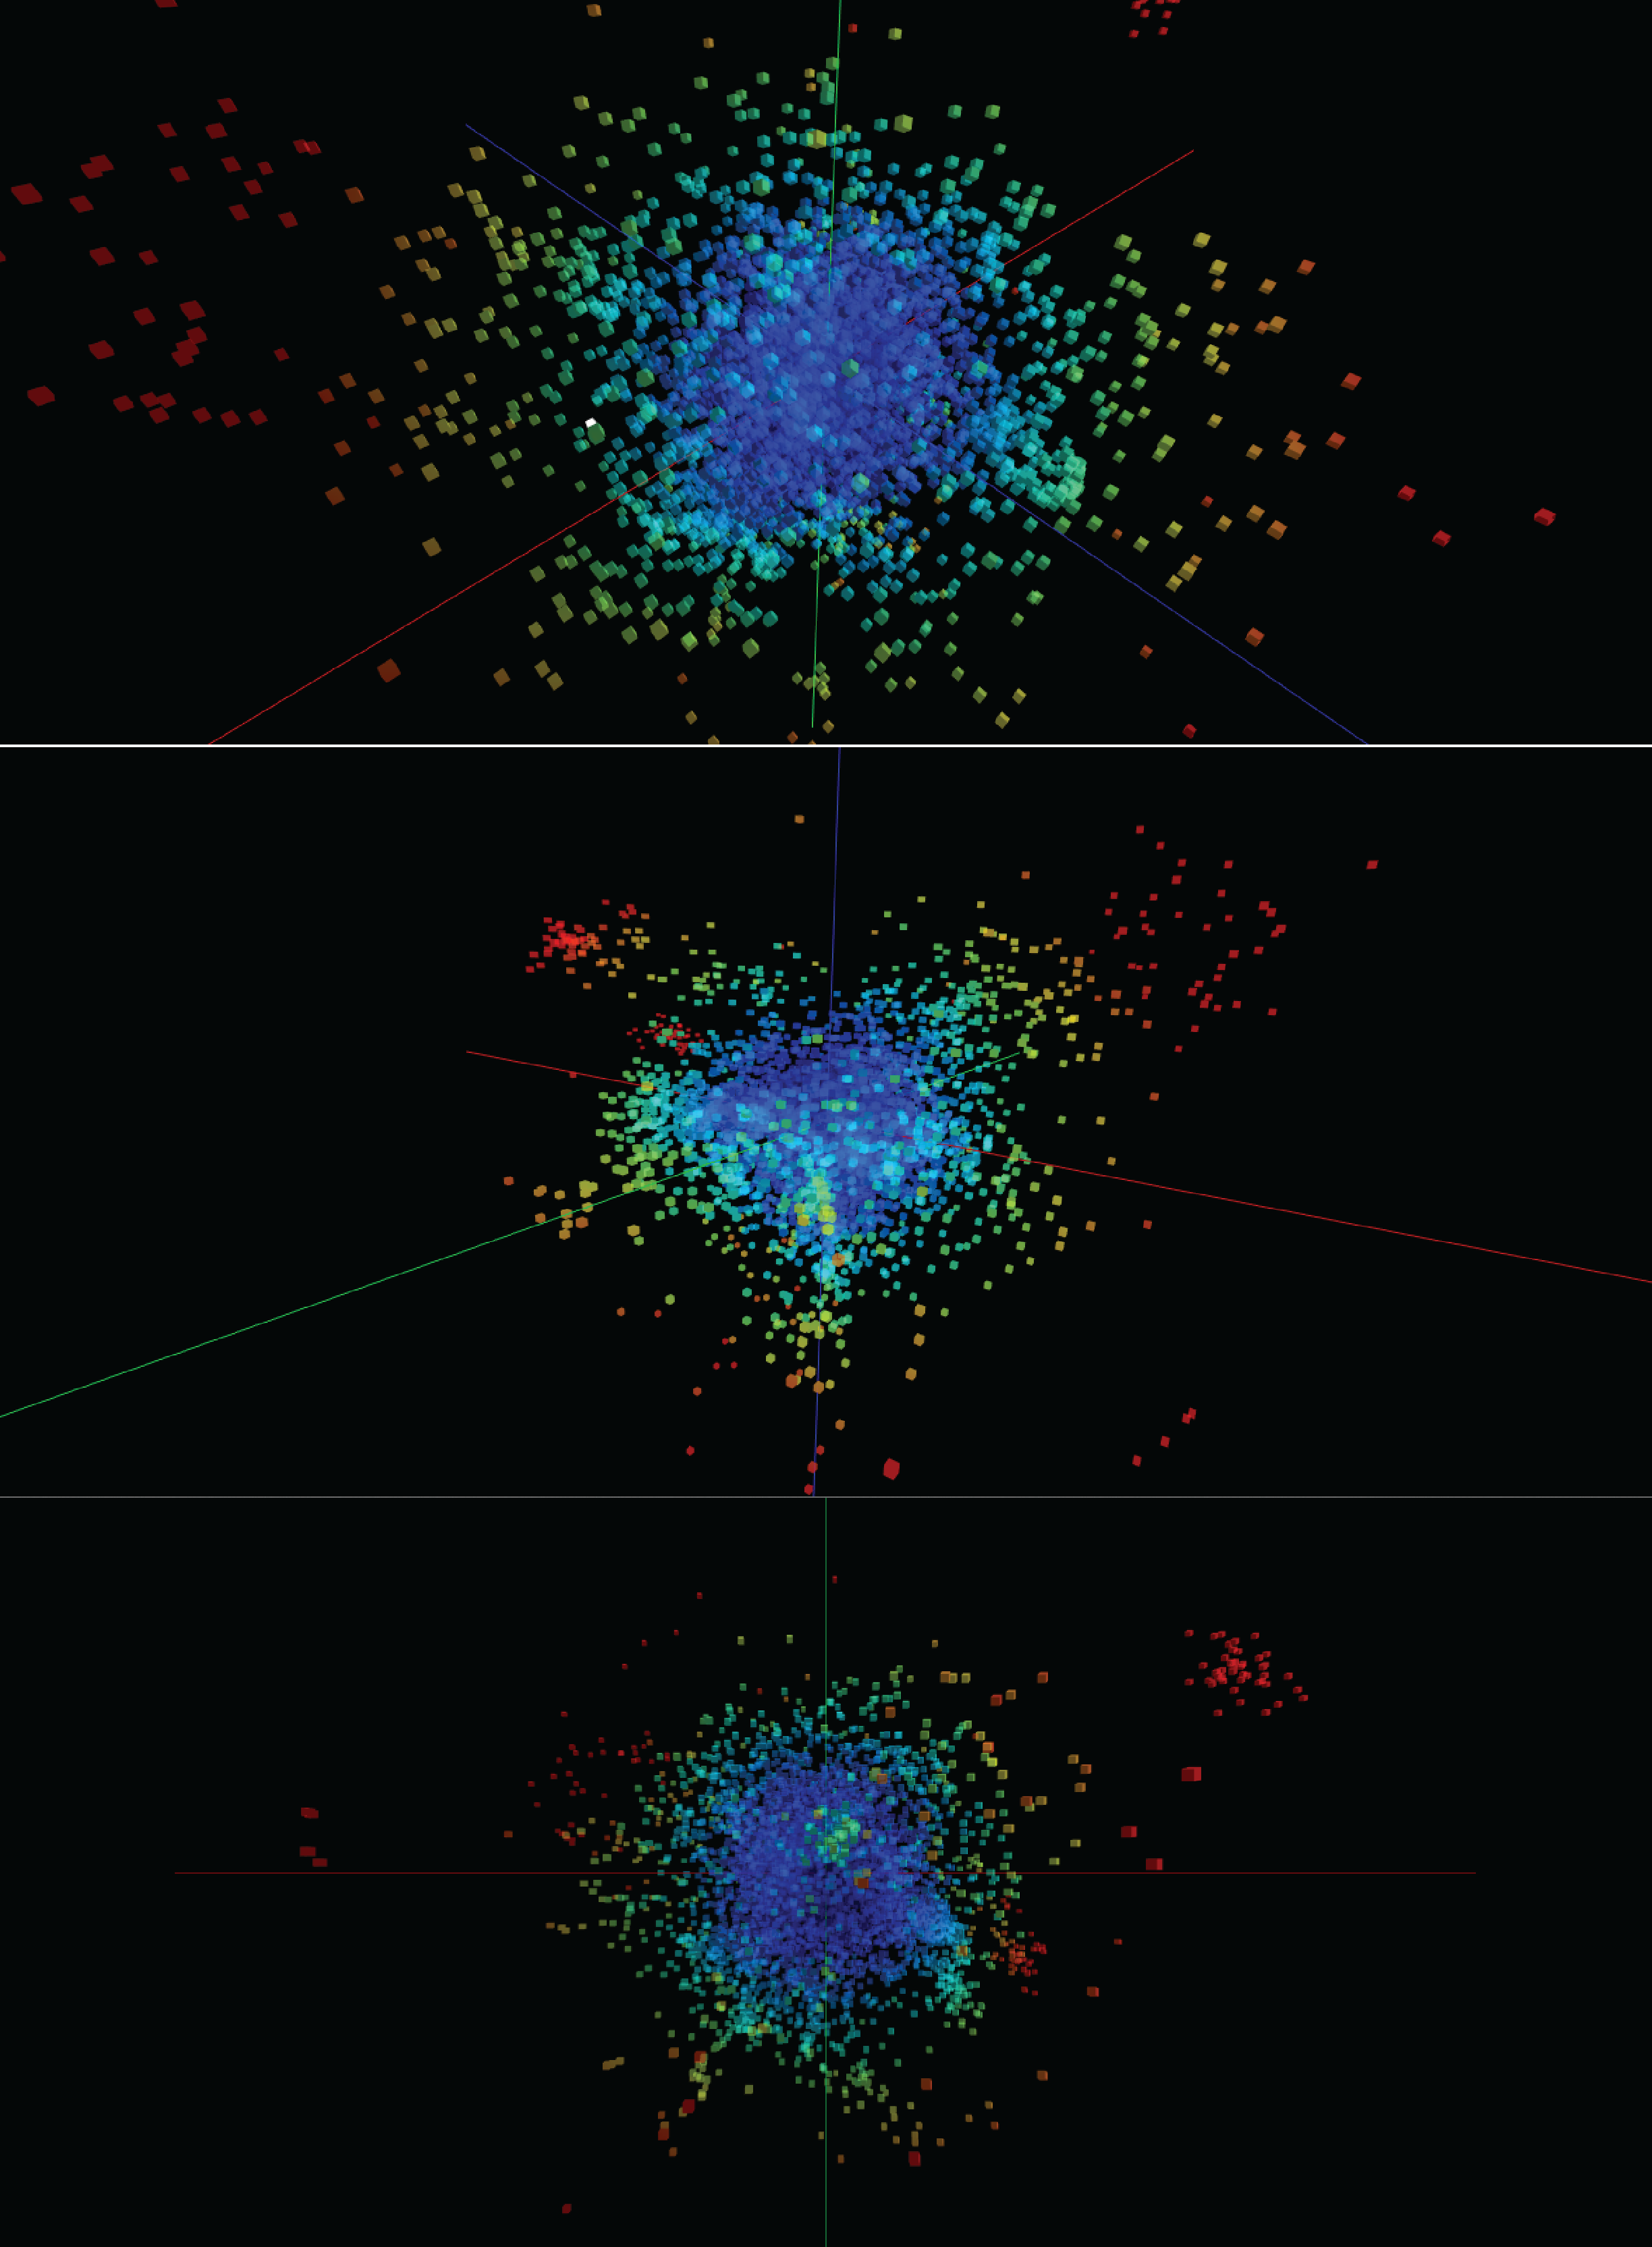
\includegraphics[width=0.38\textwidth]{images/mfcc-all.png}
  \caption{Screenshots of different camera views of the first 3 dimensions of the MFCC model visualized in the browser.  We show three different views here.}
  \label{fig:mfcc}
\end{figure}


%Describe the results of the user studies and how this resulted in changes to the interface.
%Describe that the MFCC model made a far worse visualisation according to the users. DONT discuss why yet.
%Describe how the users responded to those changes
%Detail a few areas where new information was gathered about the recordings.
%Describe how some of our metadata was verified and more clearly understood - we found components relating to Daphne Oram's piece "Birds of Parallax".

\section{Discussion and Future Work}\label{discussion}

Each researcher had prior knowledge of many aspects of the Archive and Daphne Oram's composition techniques, and were also familiar with many of the recordings.  Their interests in the archive stemmed from her methods in composition to the actual electronics of the Oramics Machine.  When given the chance to navigate the archive in a 3D space arranged by acoustic similarity, each user was incredibly pleased by the possibilities and results of just one hour's navigating, and also preferred the PLCA model to the MFCC one generally for 3 reasons: (1) the visual form and structure of the PLCA model was easier to navigate, as knowing where one was in 3D space is easier to notice, (2), navigating within the ''glob-like'' mass of the MFCC representation in 3D required users to go inside the sphere, making interaction very difficult, and (3), the mapping and clustering in the PLCA model appeared more intuitive, with users reporting they understood how it was mapped and the similarity of sounds along a projection seemed to cluster sounds better.  

Regarding (1) and (2), the form of the PLCA model (see Figure \ref{fig:plca}) is a result of the probabilistic nature of the component weights needing to sum to 1.  In 3D space, this space is defined by a 3-simplex or tetrahedron.  In comparison, MFCCs may have energy explained in all bands as there is no normalization procedure.  Plotting the first three dimensions of the MFCC model thus produces similar distributions of energy in all dimensions, creating what users called both a ``glob like'' and ``blob like'' sphere (see Figure \ref{fig:mfcc}).    Navigating inside and around a sphere presents unique challenges for a 3D browser, namely, it is difficult to select elements within the sphere and understanding the orientation of the sphere is difficult as there are no identifying features.  Thus, exploring visualizations in 3D seems to require landmarks for useful navigation.  In regards to point (3), this may be due to the greater classification and recognition performance of PLCA over MFCCs (left out for blind-review).  

Further work should focus on issues with navigating in 3D space, as some users reported on the 3D nature as requiring practice to navigate.  One solution may be to create more intuitive control through the use of other input and display devices such as touch-screens.  As well, similar latent-analysis techniques may be applied for additional meta-data from the archive as is done in audiovisual and text corpora, e.g. \cite{Himmel1998,Christel1998}, to create more informed visualizations.  In this case, the input of text annotations as well can create a user-guided visualization, where feedback from the user reshapes the 3D visualization. 

% interface, touchtable, haptics, wiimote guys
% better model selection
% exploring som versus mds...
% large databases